\documentclass[11pt]{article}
\usepackage[margin=2.3cm]{geometry}
\usepackage{graphicx,booktabs,amsmath,amssymb,siunitx,hyperref,xcolor,enumitem,caption}
\hypersetup{colorlinks=true,linkcolor=blue!50!black,urlcolor=blue!50!black,citecolor=blue!50!black}
\captionsetup{font=small}
\setlist{nosep,leftmargin=1.4em}
\newcommand{\CERT}{\textsc{[certain]}}
\newcommand{\LIK}{\textsc{[likely]}}
\newcommand{\GUESS}{\textsc{[guessing]}}
\newcommand{\NspillGood}{8,406}
\newcommand{\NspillTot}{8,443}
\newcommand{\PotGood}{4.28}
\newcommand{\BoneDx}{-0.314}
\newcommand{\BoneDxRms}{0.029}
\newcommand{\BoneDxSem}{0.0003}
\newcommand{\BoneDy}{-0.055}
\newcommand{\BoneDyRms}{0.062}
\newcommand{\SigX}{1.48}
\newcommand{\SigY}{1.48}
\newcommand{\PosX}{+0.34}
\newcommand{\PosXrms}{0.025}
\newcommand{\PosY}{-0.95}
\newcommand{\PosYrms}{0.18}
\newcommand{\HornI}{-200.5}
\newcommand{\Bxone}{+0.077}
\newcommand{\Bfracone}{16.29}
\newcommand{\Bxtwo}{+0.309}
\newcommand{\Bfractwo}{16.60}
\newcommand{\Bxthree}{+0.378}
\newcommand{\Bfracthree}{16.62}
\newcommand{\Bxfour}{+0.425}
\newcommand{\Bfracfour}{17.01}
\newcommand{\Bxfive}{+0.404}
\newcommand{\Bfracfive}{16.93}
\newcommand{\Bxsix}{+0.437}
\newcommand{\Bfracsix}{16.55}
\newcommand{\LevBoneXhalf}{-0.055}
\newcommand{\LevRestXhalf}{-0.092}
\newcommand{\LevRestYhalf}{-0.293}
\newcommand{\LevD}{-0.387}
\newcommand{\PredAzero}{+0.24}
\newcommand{\PredAmone}{+1.74}
\newcommand{\PredAone}{-0.89}
\newcommand{\Curv}{0.0203}
\newcommand{\Rone}{0.982}
\newcommand{\Rtwo}{0.909}
\newcommand{\Rthree}{0.753}
\newcommand{\Rfourhalf}{0.440}
\newcommand{\MinDeltaOneEfive}{2.5}
\newcommand{\MinDeltaOneEsix}{0.80}
\newcommand{\ScanFifty}{0.27}
\newcommand{\ScanTwoH}{0.14}
\newcommand{\ScanFiveH}{0.09}
\newcommand{\ScanTwoK}{0.04}
\newcommand{\NarrowTwoKfail}{25}
\newcommand{\NarrowTwoKrms}{0.83}
\newcommand{\WrongBias}{-0.06}
\newcommand{\CountsQuarter}{59}
\newcommand{\CountsHalf}{16}
\newcommand{\CountsTenth}{400}
\newcommand{\BRspills}{451}
\newcommand{\BRtrig}{454}
\newcommand{\BRunmatched}{0}
\newcommand{\BRdropT}{1}
\newcommand{\BRdropGB}{2}
\newcommand{\BRdropDup}{0}
\newcommand{\BRoffset}{13.0}
\newcommand{\BRresid}{2.8}
\newcommand{\BRtone}{1310}
\newcommand{\BRflashes}{693}
\newcommand{\BRratio}{1.069}
\newcommand{\BRerr}{0.113}
\newcommand{\BRpval}{0.52}
\newcommand{\BRmindelta}{31}
\newcommand{\BRnone}{107}
\newcommand{\BRnrest}{547}
\newcommand{\FRperSpill}{1.51}
\newcommand{\FRperEthirteen}{0.298}
\newcommand{\FRrockPerSpill}{0.24}
\newcommand{\FRspillPot}{5.07}
\newcommand{\FRpowerKw}{812}
\newcommand{\FRperHourScan}{510}
\newcommand{\FRrockPerHourScan}{81}
\newcommand{\FRrunOneTotal}{6.6\times10^{5}}
\newcommand{\FRrunOneMinDelta}{1.0}
\newcommand{\THalfAll}{2\,min}
\newcommand{\THalfRock}{12\,min}
\newcommand{\THalfNu}{19\,min}
\newcommand{\TQuarterAll}{7\,min}
\newcommand{\TQuarterRock}{43\,min}
\newcommand{\TQuarterNu}{70\,min}
\newcommand{\TTenthAll}{47\,min}
\newcommand{\TTenthRock}{4.9\,h}
\newcommand{\TTenthNu}{8.0\,h}

\graphicspath{{../results/}}
\title{NuMI proton-beam position on target versus 2x2 / Mx2 rates:\\
Run~1 proof of concept and target-scan feasibility}
\author{Prepared for J.~L.~Barrow (UMN) with Claude (Anthropic)\\
\small Builds on the \texttt{beam\_quality} package of G.~Ingratta and B.~Howard (York U.)}
\date{11 November 2026\\ \small code: \texttt{joshuabarrow221/arcube\_nearline}, branch \texttt{claude/project-thread-e9bc00}, dir \texttt{beam\_position\_scan/}}
\begin{document}
\maketitle

\noindent Confidence tags: \CERT{} = measured here from data or exact arithmetic;
\LIK{} = strong inference from data plus standard physics; \GUESS{} = filling a gap,
must be checked.

\section{Executive summary}
\begin{enumerate}
\item \textbf{Run~1 cannot pinpoint an ``optimal'' beam position, and the batch-split
test is expected to come out null.} Batch~1 is displaced by \BoneDx\,mm in $x$
(RMS \BoneDxRms\,mm spill to spill) and \BoneDy\,mm in $y$ relative to batches 2--6 \CERT.
Against a \SI{7.4}{mm}-wide target fin and a $\sigma_x=\SigX$\,mm beam this changes the
fraction of protons hitting the fin by only \PredAzero\% if the beam sits at the
BPM-coordinate origin, and by \PredAmone\% / \PredAone\% if the fin centre is
\SI{1}{mm} to either side \LIK. Run~1 should yield $\sim\!\FRrunOneTotal$ selected in-spill
light flashes (projected from the 19-file rate, \LIK), enough to see a \FRrunOneMinDelta\% batch-1/batches-2--6 difference at
$3\sigma$. The batch split can therefore only flag a beam that was $\gtrsim1$\,mm off the
fin centre in $x$. It cannot locate an optimum. Measured on \BRspills{} spills from
\BRfiles{} files: $R_1/R_{2\text{--}6}=\BRratio\pm\BRerr$ for all flashes and
$\BRtwoRatio\pm\BRtwoErr$ for flashes lighting $\geq$2 TPCs. Both are null, as predicted
\CERT.
\item \textbf{Halving or quartering the batch ``ellipses'' adds nothing in $x$.} The beam is
extremely steady in $x$ (spill RMS \PosXrms\,mm), so splitting each batch population at its
median gives a lever arm of only \LevBoneXhalf\,mm (batch~1) and \LevRestXhalf\,mm
(batches 2--6) \CERT. In $y$ the halves differ by \LevRestYhalf\,mm, but the fin is
\SI{63}{mm} tall, so interception has no $y$ dependence there. Any $y$ effect would come
from horn focusing alone, which is much weaker \LIK.
\item \textbf{The batch comparison is confounded by time order, and the bias is bigger than
the signal.} Batch~1 is always first in the spill. Delayed ``follower'' flashes from earlier
interactions ($\tau\approx\FBtau\,\mu$s, consistent with stopped-muon decays) pile into the
later batches and never into batch~1. Measured from the post-spill tail, this biases
$R_1/R_{2\text{--}6}$ by \FBbias\% for all flashes and \FBtwoBias\% for flashes lighting
$\geq$2 TPCs \LIK. Both are larger than the $\sim$0.2\% interception signal expected for a
centred beam. No pile-up \emph{loss} is seen: later batches have, if anything, more flashes
after an earlier one (batch~6: $\MaskSix\pm\MaskSixErr$) (\S\ref{sec:syst}).
\item \textbf{A dedicated horizontal scan that reaches the fin edges is feasible with the
2x2 light system at \SI{100}{kW}.} The measured in-spill flash rate is \FRperEthirteen{}
flashes per $10^{13}$\,POT ($\approx$\FRperSpill{} per spill at \FRpowerKw\,kW). That
corresponds to $\approx$\FRperHourScan{} flashes per hour at \SI{100}{kW}, about ten times
the $\sim$50 neutrinos/hour assumed in the email thread. With \CountsQuarter{} counts per
point, a 7-point scan over $\pm$4.5\,mm locates the fin centre to $\pm$0.25\,mm
(statistical), and about \CountsTenth{} counts per point gives $\pm$0.1\,mm (toy MC).
That is roughly \TQuarterAll{} and \TTenthAll{} per point, respectively, using all flashes. A plateau scan
($\pm$1\,mm about nominal) does not converge even with 2000 counts per point
(\NarrowTwoKfail\% of toys find no maximum) \LIK.
\item \textbf{The detector can confirm the target centre. It is not competitive with the
accelerator's own instruments for optimisation.} NuMI's beam-based alignment reaches
$\sim$\SI{0.03}{mm} with profile monitors and $\sim$\SI{0.26}{mm} with BPMs, and uses
hadron and muon monitors with $10^{6\text{--}8}$ particles per spill
\cite{zwaska2006}. The useful product of a 2x2 scan is an independent,
neutrino-side check that the rate-weighted target centre agrees with the BPM centre.
\item \textbf{Run~1 was taken in reverse horn current (antineutrino mode)}
\cite{nufact2024}, yet the \texttt{beam\_quality} horn cut ($-202<I<-196.4$\,kA,
documented as FHC) passes every Run~1 spill with $I\approx\HornI$\,kA. The stripline sum
evidently does not encode polarity. The package README's statement that the 2024 data
are ``nominal FHC running'' is therefore probably wrong \LIK. This does not affect the
position analysis, but it should be fixed before the horn cut is used to classify
polarity.
\end{enumerate}

\section{Question, hypotheses, and what was tested}
The request: determine how the proton-beam position on the NuMI target affects the rates
seen in 2x2 and Mx2, whether ``optimal'' positions can be pinpointed, and whether past
data can confirm the approach. The proposed proof of concept uses batch~1 (``not as
kicked'') and batches 2--6 as two simultaneous beam positions, subdivides them if
statistics allow, and extrapolates to $\sim$\SI{100}{kW} with $\sim$\SI{1}{h} per position.

\paragraph{Where the premise holds and where it does not.}
\begin{itemize}
\item Using batches as simultaneous positions is a good idea. Every detector, live-time,
purity and beam-intensity condition is shared, so only the position (and the time order,
\S\ref{sec:syst}) differ. The data support this: the offset is real, stable and
measured spill by spill (\S\ref{sec:beam}).
\item I disagree that the neutrino-optimal position is where ``true vertices are directly on
axis.'' A sub-mm parallel displacement at the target moves the neutrino-beam centre at
\SI{1}{km} by the same sub-mm amount. That is invisible against a beam several metres
wide. What changes the rate is (a) the fraction of protons intercepted by the fin and
(b) the horn-focusing acceptance for secondaries made off axis.
Here's what I'd do instead: define the optimum operationally as the centre of the
rate-versus-position response, found from its edges.
The risk in your approach is chasing a maximum on a plateau that is flat to
$<$1\% over $\pm1$\,mm (\S\ref{sec:model}).
\item I disagree that rock-muon rates are an uncontroversial proxy for the neutrino rate in
this context. Rock muons are weighted toward higher neutrino energies, whose parents are
less affected by horn focusing than the flux peak. Interception changes affect both
equally, so an edge scan works with either. For focusing-driven changes near the
optimum, the two proxies can disagree \LIK.
Here's what I'd do instead: report the fully contained, rock-muon-like ($\geq4$ TPCs lit),
and all-flash rates separately and require them to agree.
The risk in your approach is that a combined ``neutrino-equivalent rate'' hides a
proxy-dependent optimum.
\item ``$\sim$50 neutrinos/hour/position'' undersells the detector for this purpose. The
quantity that matters is any in-spill activity whose rate is proportional to the flux:
light flashes from rock muons and neutrino interactions in and around the argon. Measured:
$\approx$\FRperHourScan/h at \SI{100}{kW} \LIK{} (one-file rate, \S\ref{sec:det}).
\end{itemize}

\section{Data and access}\label{sec:data}
\begin{itemize}
\item \textbf{Beam:} IFBeam per-spill records on TCLK \$A9 for the BPM arrays
\texttt{E:HP121[]}, \texttt{E:VP121[]}, \texttt{E:HPTGT[]}, \texttt{E:VPTGT[]} and the
intensities \texttt{E:HITGT[]}, \texttt{E:VITGT[]}. Element~0 is the auto-tune average and
elements 1--6 are batches. The two existing \texttt{get\_data.cpp} exports were used:
2024-07-09 00:00--02:05 and 2024-07-12 00:01--01:01 CDT, with \NspillTot{} spills,
\NspillGood{} of them goodbeam, and $\PotGood\times10^{17}$\,POT. The scalar spellings
(e.g.\ \texttt{E:HPTGT}) return HTTP 200 with \emph{zero rows}. Code that does not check
for empty rows silently gets nothing \CERT.
\item \textbf{2x2:} Run~1 merged charge+light FLOW, reflow v11 (flow v1.5.0), streamed by
HTTP byte ranges from \url{https://portal.nersc.gov/project/dune/data/2x2/reflows/v11/flow/beam/}.
Only \texttt{light/events}, \texttt{light/t\_ns}, \texttt{light/sum\_hits} and the event--hit
references are read; the \SI{8}{GB} of waveforms per file are not. The Run~1 RunsDB
(\texttt{mx2x2runs\_v0.2.sqlite}) gives $2.2\times10^{19}$\,POT with CRS and LRS both
recorded ($3.0\times10^{19}$ LRS only).
\item \textbf{Mx2:} MINERvA DSTs are on the portal (\texttt{data/2x2/Mx2/dst/}: 502 files,
$\sim$374\,MB each, runs 50000--50018). Each file has one tree, \texttt{minerva}, with one entry
per gate (gates 1.1997\,s apart) and per-hit \texttt{hit\_time}, \texttt{hit\_module},
\texttt{hit\_plane}, \texttt{hit\_pe}. That is enough to assign front-plane hits to batches.
File-name times are UTC \CERT. They were not analysed here; see \S\ref{sec:next}.
\item \textbf{Access constraint:} neither portal.nersc.gov nor the IFBeam API is reachable
from the cloud machine that wrote this report. All fetches ran on the requester's laptop.
The full-Run~1 extraction should run at NERSC against the files directly.
\end{itemize}

\section{Beam side: is batch 1 really somewhere else?}\label{sec:beam}
Per-batch positions at the target $z$ were obtained by the same linear extrapolation from
the 121 and TGT BPM stations used by the NOvA \texttt{BpmProjection} port in
\texttt{get\_data.cpp}. Fig.~\ref{fig:batches} and Table~\ref{tab:batches} summarise them.

\begin{figure}[h]\centering
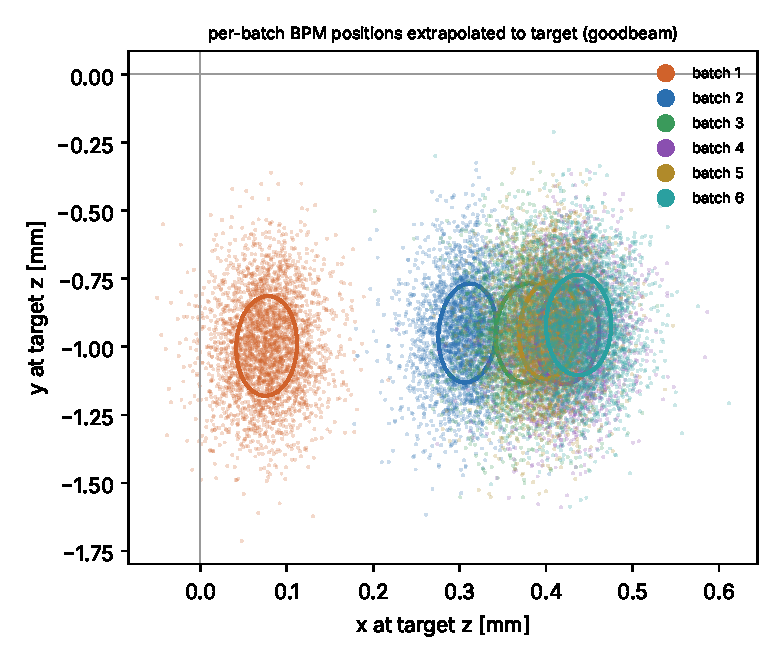
\includegraphics[width=0.48\textwidth]{ifbeam/batch_positions.pdf}\hfill
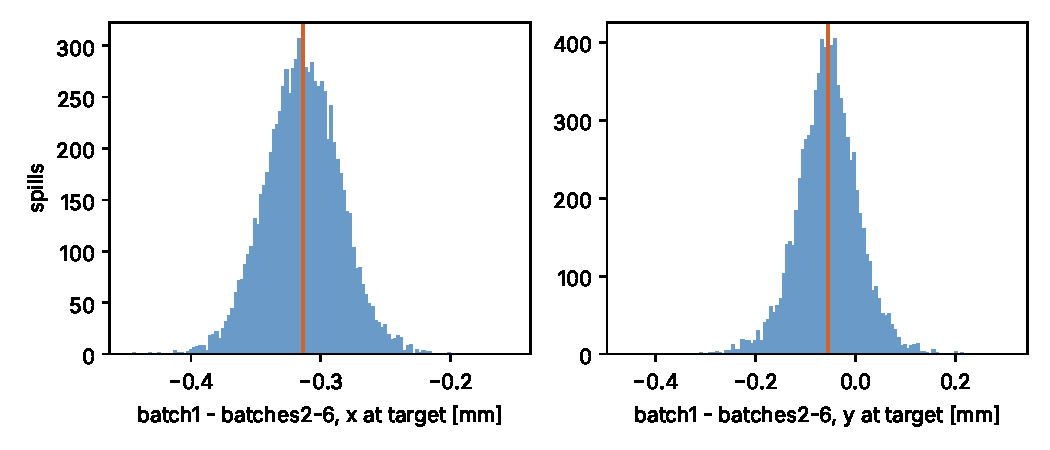
\includegraphics[width=0.48\textwidth]{ifbeam/batch1_offset_hist.pdf}
\caption{Left: per-batch BPM positions extrapolated to the target, goodbeam spills, both
windows (ellipses: $1\sigma$). Right: per-spill offset of batch~1 from the
intensity-weighted mean of batches 2--6.}\label{fig:batches}
\end{figure}

\begin{table}[h]\centering\small
\begin{tabular}{lcccccc}\toprule
batch & 1 & 2 & 3 & 4 & 5 & 6\\\midrule
$\langle x\rangle$ at target [mm] & \Bxone & \Bxtwo & \Bxthree & \Bxfour & \Bxfive & \Bxsix\\
intensity share [\%] & \Bfracone & \Bfractwo & \Bfracthree & \Bfracfour & \Bfracfive & \Bfracsix\\\bottomrule
\end{tabular}
\caption{Per-batch means. Statistical errors on the means are $<$0.001\,mm.}\label{tab:batches}
\end{table}

Findings \CERT:
\begin{itemize}
\item Batch~1 minus batches 2--6: $\Delta x=\BoneDx\pm\BoneDxSem$\,mm (RMS \BoneDxRms),
$\Delta y=\BoneDy$\,mm (RMS \BoneDyRms). The offset is constant to $\pm0.01$\,mm across
10-minute blocks spanning both days.
\item Batches 2--6 are not one position either. They drift monotonically by
$\sim$0.13\,mm in $x$ from batch~2 to batch~6, consistent with a sagging kicker flat-top.
\item Batch~1 carries less beam (\Bfracone\% of the spill against $\sim$16.6--17.0\%), so
rates must be per POT \emph{per batch}.
\item Spill-to-spill jitter is tiny in $x$ (RMS \PosXrms\,mm) and larger in $y$
(\PosYrms\,mm). Beam width from the multiwire: $\sigma_x=\SigX$, $\sigma_y=\SigY$\,mm.
\end{itemize}
The batch offset is \emph{larger} than the jitter, so it is the only usable $x$ lever arm
in normal running. It is a fifth of the beam width and a twentieth of the fin width.

\section{Rate model}\label{sec:model}
The only position dependence computable without a beamline simulation is interception.
For a Gaussian beam of RMS $\sigma$ centred at $x_0$ from the centre of a fin of full width
$w$,
\[ f(x_0)=\Phi\!\left(\tfrac{w/2-x_0}{\sigma}\right)-\Phi\!\left(\tfrac{-w/2-x_0}{\sigma}\right),\qquad
\frac{f(x_0)}{f(0)}\simeq1-k\,x_0^2,\quad k=\frac{w/\sigma^3\,\phi(w/2\sigma)}{2f(0)}=\Curv~\text{mm}^{-2}. \]
Protons that miss the fin are given a relative neutrino yield $\epsilon=0.2$ (\GUESS;
results below are insensitive to it). With $w=\SI{7.4}{mm}$ (the NOvA-era ME fin
\cite{numi_target}; the 1\,MW-era fin width was not confirmed, \GUESS) and $\sigma=\SigX$\,mm
the relative rate is \Rone{} at 1\,mm, \Rtwo{} at 2\,mm, \Rthree{} at 3\,mm and \Rfourhalf{}
at 4.5\,mm (Fig.~\ref{fig:model}).
For scale, the 2005 NuMI beam-based alignment quotes $\sim$2\% spectral distortions for
$\sim$1\,mm target/baffle offsets in the low-energy configuration \cite{zwaska2006}.
Focusing effects of that size are not in this model. They need g4numi derivatives for the
present configuration, which would replace the free quadratic term in
\texttt{target\_model.relative\_rate}.

\begin{figure}[h]\centering
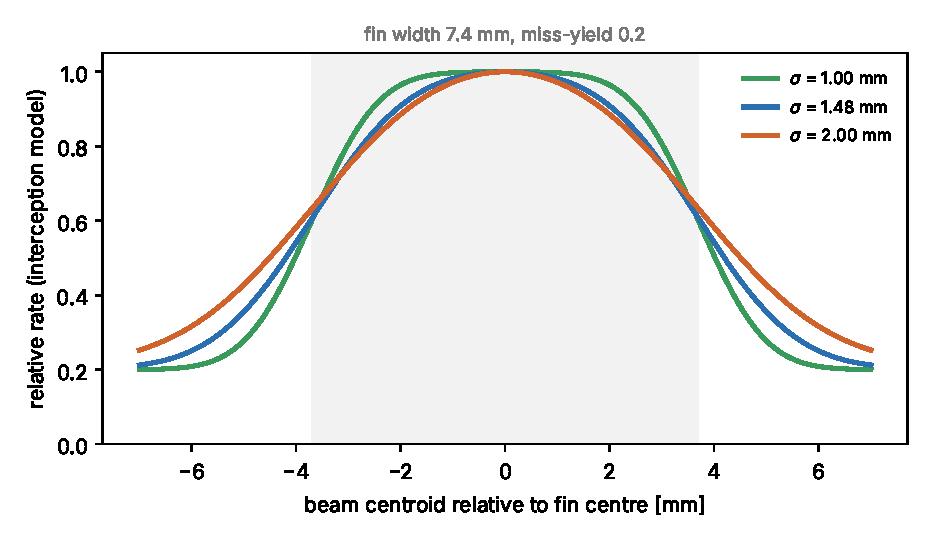
\includegraphics[width=0.6\textwidth]{sensitivity/intercept_response.pdf}
\caption{Relative rate versus beam offset from the fin centre (interception model). The
shaded band is the fin.}\label{fig:model}
\end{figure}

\section{Detector side: per-batch light-flash rates}\label{sec:det}
\paragraph{Why light, not charge.} CRS timestamps are smeared by drift times of up to
$\sim$\SI{200}{\micro s}, so a charge cluster cannot be assigned to a \SI{1.58}{\micro s}
batch without an external $t_0$. The LRS digitises a \SI{16}{\micro s} window opened by the
beam trigger at \SI{16}{ns} per sample, so each pulse's time relative to the trigger is
known to $\sim$10--20\,ns \CERT. The spill appears as a $\approx$\SI{9.5}{\micro s} plateau
starting $\approx$\BRtone\,ns after the trigger (Fig.~\ref{fig:flash}).

\paragraph{Selection.}
\begin{enumerate}
\item Beam triggers are \texttt{light/events} with \texttt{trig\_type}=1. In the file
checked, 454 such triggers matched 455 IFBeam spills; this mapping is not documented
(\LIK).
\item Spill matching uses the light DAQ unix time: trigger $-$ \$A9 $=\BRoffset$\,ms, RMS
\BRresid\,ms. Spills with $|$residual$|>10$\,ms are dropped as timing drifts, per the
requirement to remove rather than correct such events.
\item Summed-channel hits (\texttt{sum\_hits}) are timed with \texttt{busy\_ns}+\texttt{ns\_spline}.
The \texttt{ns} field is the \emph{event} time stored as float64 ($\sim$256\,ns precision at
$1.7\times10^{18}$), not the hit time \CERT. Hits within 80\,ns are merged across all TPCs
into flashes, so a through-going muon counts once. Flashes need $\geq3$ hits.
\item The batch-1 start is fitted from the data; six nominal batches of 84 RF buckets
(\SI{1581.8}{ns}) follow. Guard bands of 50\,ns (100\,ns around batch~1) are removed and
the POT is scaled by the surviving fraction of each batch.
\end{enumerate}

\paragraph{Result (\BRfiles{} files: 2024-07-09 23:54--02:05 and 2024-07-12 00:00--01:00 CDT, runs 50017/50018).}
\BRtrig{} beam triggers; \BRunmatched{} unmatched, \BRdropT{} dropped for timing,
\BRdropDup{} duplicate matches and \BRdropGB{} not goodbeam, leaving \BRspills{} spills and
\BRflashes{} selected flashes. Batch~1 / batches 2--6 per-POT rate ratio:
\[ R_1/R_{2\text{--}6}=\BRratio\pm\BRerr\quad(p=\BRpval), \]
with \BRnone{} and \BRnrest{} flashes. The $3\sigma$ reach of this subsample is
\BRmindelta\%, an order of magnitude above the $\sim$0.2\% expected for a centred beam.
In the interception model ($\sigma=1.48$\,mm, $w=7.4$\,mm) a ratio this far from unity
needs the fin centre $\gtrsim$3\,mm from the beam, so this sample excludes only a gross
miss \LIK. The full Run~1 sample (reach $\approx$1\%) would reach $\approx$1\,mm. Requiring $\geq$2 lit TPCs
(which suppresses single-TPC followers) gives $\BRtwoRatio\pm\BRtwoErr$ from \BRtwoN{} flashes.
Correcting each for the follower bias gives \BRcorr{} and \BRtwoCorr{}, respectively.

\paragraph{The batch edges are visible in the data.} The flash-time distribution
(Fig.~\ref{fig:flash}) has narrow dips at the fitted batch boundaries: the empty RF buckets
between Booster batches. So the batch assignment is checked by the data themselves, not
only by the 84-bucket arithmetic \CERT.

\paragraph{Data defect: duplicated light events.} Two of the \BRfiles{} v11 files
(\texttt{packet-0050017-2024\_07\_09\_01\_14\_40} and \texttt{packet-0050018-2024\_07\_12\_00\_00\_19})
contain repeated light triggers: 687 and 456 beam triggers, respectively, share an
IFBeam spill with another trigger. All \BRdropDup{} such triggers were dropped, together
with the spills they matched, rather than guessing which copy is real. This should go to the reflow
maintainers \CERT.

\begin{figure}[h]\centering
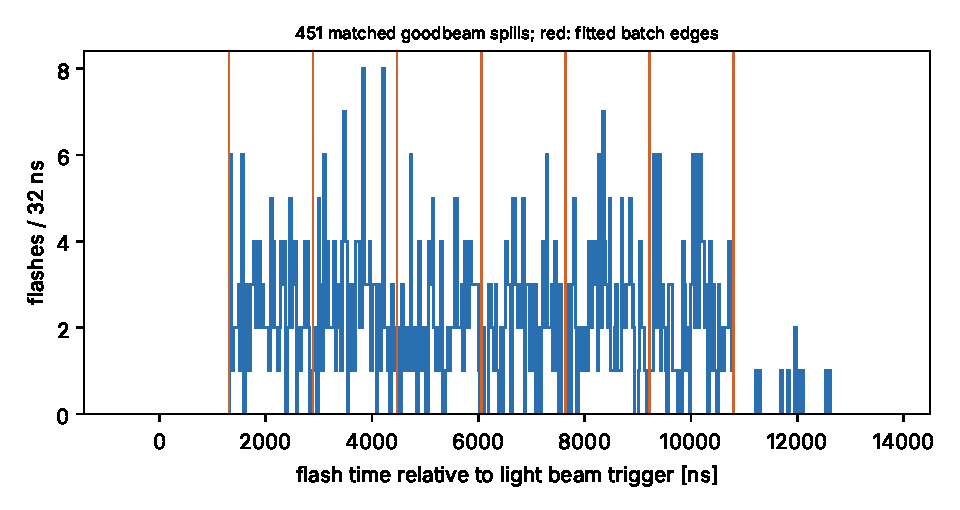
\includegraphics[width=0.62\textwidth]{batch_rates/flash_times.pdf}\hfill
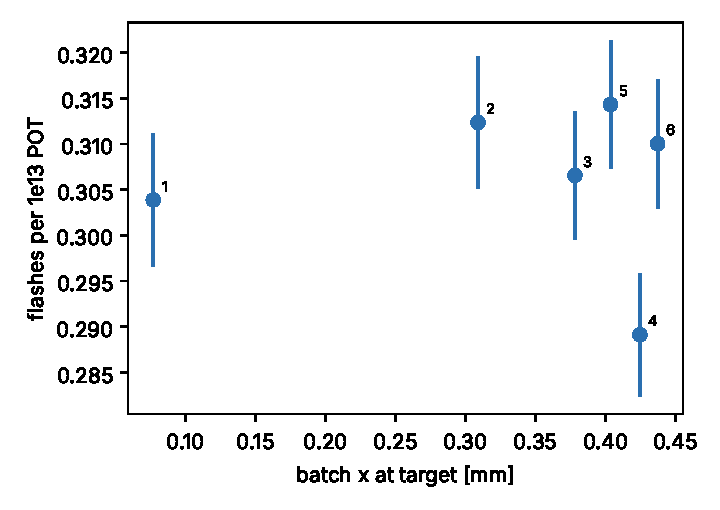
\includegraphics[width=0.36\textwidth]{batch_rates/rate_vs_batch_x.pdf}
\caption{Left: flash times relative to the light beam trigger, with the fitted batch edges.
Right: per-POT flash rate per batch against that batch's mean $x$ at the target.}\label{fig:flash}
\end{figure}

\section{Sensitivity and extrapolation}\label{sec:sens}
\paragraph{Batch split, Run~1.} With a fraction $\varphi=1/6$ of the POT in batch~1, a
fractional difference $\delta$ is seen at $Z\sigma$ when
$N_\text{tot}\geq Z^2\delta^{-2}(\varphi^{-1}+(1-\varphi)^{-1})=7.2Z^2/\delta^2$ (verified by
toys in \texttt{tests/}). The measured flash rate projects to $\approx\FRrunOneTotal$ selected
flashes for the $2.2\times10^{19}$\,POT with CRS+LRS live, giving a \FRrunOneMinDelta\%
$3\sigma$ reach (Fig.~\ref{fig:reach}). The model predicts $|\delta|\gtrsim1$\% only if the
fin centre is $\gtrsim$1\,mm from the beam in $x$. A further 0.3\% per-batch POT-share
uncertainty (BPM intensities used as weights) is included in the dashed curve.

\begin{figure}[h]\centering
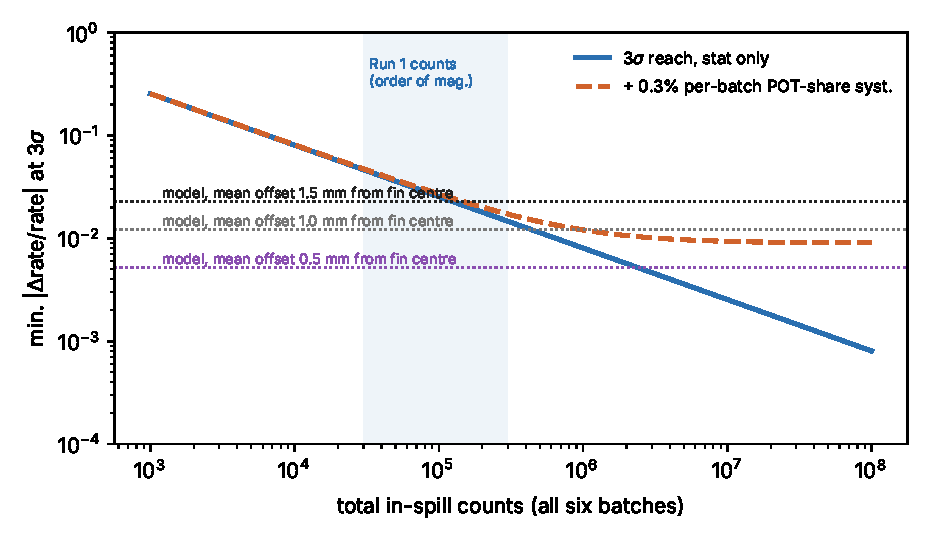
\includegraphics[width=0.49\textwidth]{sensitivity/batch_split_reach.pdf}\hfill
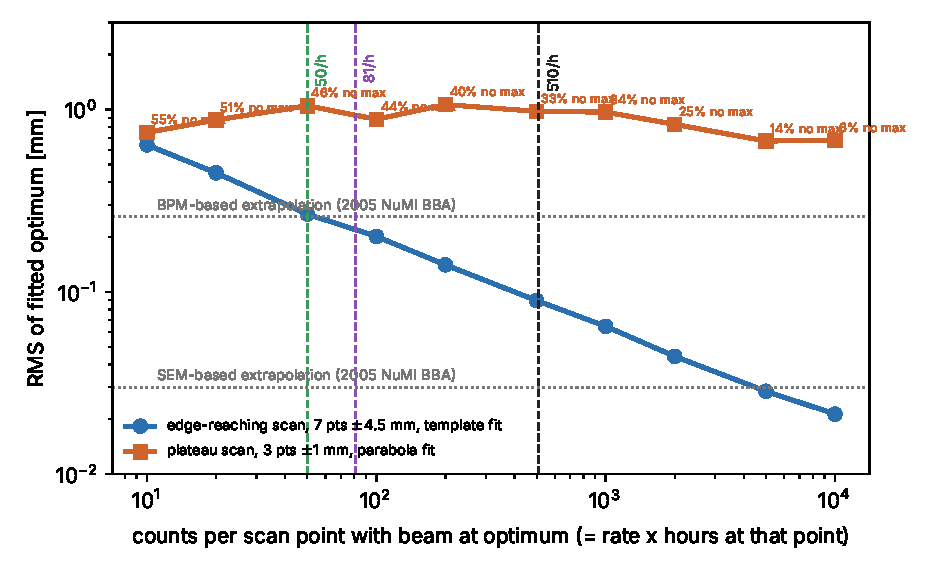
\includegraphics[width=0.49\textwidth]{sensitivity/scan_precision.pdf}
\caption{Left: $3\sigma$ reach of the batch-1 versus batches-2--6 comparison against total
counts, with model predictions for different fin-centre offsets. Right: toy-MC precision on
the fitted optimum against counts per scan point. The dashed verticals mark assumed hourly
rates at 100\,kW; the measured rate is $\approx$\FRperHourScan/h.}\label{fig:reach}
\end{figure}

\paragraph{Dedicated scan at 100\,kW.} Detector rates scale with POT. At \SI{100}{kW} with
a \SI{1.2}{s} cycle and 46 spills per 60.46\,s supercycle, the flash yield is
$\approx$\FRperHourScan/h for all selected flashes and $\approx$\FRrockPerHourScan/h for
flashes lighting $\geq$4 TPCs (rock-muon-like). Toy-MC results for a 7-point scan over
$\pm$4.5\,mm with a template fit of the known shape:

\begin{center}\small
\begin{tabular}{lccc}\toprule
target precision on fin centre & 0.5\,mm & 0.25\,mm & 0.1\,mm\\\midrule
counts per point (at optimum) & \CountsHalf & \CountsQuarter & \CountsTenth\\
time per point, all flashes ($\approx$\FRperHourScan/h) & \THalfAll & \TQuarterAll & \TTenthAll\\
time per point, $\geq$4 TPCs ($\approx$\FRrockPerHourScan/h) & \THalfRock & \TQuarterRock & \TTenthRock\\
time per point, contained $\nu$ ($\sim$50/h, email estimate) & \THalfNu & \TQuarterNu & \TTenthNu\\\bottomrule
\end{tabular}\end{center}

\noindent Fitting with a deliberately wrong template ($\sigma$ 30\% too large and
$\epsilon=0$) shifts the centre by only \WrongBias\,mm, because a symmetric shape error does
not move the centre \LIK. A $\pm$1\,mm plateau scan fails even at 2000 counts per point:
\NarrowTwoKfail\% of toys have no maximum, and the rest scatter by \NarrowTwoKrms\,mm.
\textbf{One hour per position at 100\,kW is enough if, and only if, the scan reaches the fin
edges.} Whether running the beam onto the fin edge at 100\,kW is acceptable (baffle and
fin-edge heating) is the accelerator's call.

\section{Systematics and caveats}\label{sec:syst}
\begin{itemize}
\item \textbf{Time-order bias in the batch split.} Two opposite effects are possible:
masking (an earlier flash hides a later one) and followers (an earlier interaction adds a
delayed flash). The data show followers dominating. The post-spill tail decays with
$\tau\approx\FBtau\,\mu$s, and the steady-state follower fraction is \FBf\% of in-spill
flashes (\FBtwoF\% with $\geq$2 TPCs). The expected follower share rises from batch~1 to
batch~6, biasing $R_1/R_{2\text{--}6}$ by \FBbias\% (\FBtwoBias\%). The tail fit uses only
$\sim$100 flashes, so these corrections are uncertain at the $\sim$30--50\% level \LIK.
\texttt{detector\_rates.follower\_bias} implements the estimate. The scan is not affected,
because position does not correlate with time order there.
\item \textbf{Per-batch POT.} The batch shares come from BPM intensities, not toroids.
A 0.3\% share error is already comparable to the expected signal.
\item \textbf{Trigger identity.} \texttt{trig\_type}=1 was matched to IFBeam counts in one
file only. Confirm it with the LRS configuration.
\item \textbf{Horn polarity labelling} (summary item 6).
\item \textbf{Vertical plane.} The fin is tall, so a vertical scan has no edges within a
safe range. Any vertical optimisation relies on focusing effects of order 1\%/mm.
\item \textbf{Fin width at 1\,MW.} The 7.4\,mm value is for the NOvA-era ME target. The
centre found by an edge scan does not depend on it; the predicted batch-split size does.
\end{itemize}

\section{Recommendations and next steps}\label{sec:next}
\begin{enumerate}
\item Tell the accelerator team: the 2x2 can provide an independent, neutrino-side
measurement of the horizontal target centre to $\sim$0.1--0.25\,mm in a 7-point,
$\pm$4.5\,mm scan at 100\,kW with \TQuarterAll--\TTenthAll{} per point (all flashes) or \TQuarterRock--\TTenthRock{} (rock-muon-like only). That holds if they can sit at
those offsets, and the scan time is driven by their safety limits rather than our
statistics. Do not offer to find a rate maximum on the plateau.
\item Ask for the scan's per-setpoint BPM targets and timestamps in IFBeam (the existing
\texttt{[]} devices suffice). No new ACNET parameters are needed for our side.
\item Run \texttt{extract\_lrs\_flashes.py} on all Run~1 v11 files \emph{at NERSC} (local
filesystem, no streaming), fetch per-batch IFBeam data for the same span, and run
\texttt{batch\_rates.py}. Include the pile-up study before quoting a ratio.
\item Mx2: write a DST reader that emits (spill time, hit time relative to gate) for the
front planes, and feed it to \texttt{detector\_rates}. MINERvA timing ($\sim$ns) resolves
batches as well. It adds an independent rock-muon sample with different acceptance.
\item Obtain g4numi derivatives of the 2x2 flash and contained-$\nu$ rates with respect to
beam $x$, $y$ and angle for the current target and horns. They replace the
interception-only model before any scan decision.
\end{enumerate}

\section{Reproduction}
See \texttt{beam\_position\_scan/README.md}. In short:
\begin{verbatim}
python3 scripts/analyze_ifbeam_batches.py STEM1 STEM2 --out results/ifbeam
python3 scripts/sensitivity_study.py --sigma 1.48 --width 7.4
python3 scripts/extract_lrs_flashes.py --out flashes/ <FLOW files or URLs>
python3 scripts/batch_rates.py --flashes flashes/*.npz --ifbeam STEM1 STEM2 \
        --out results/batch_rates
python3 scripts/make_report_numbers.py && cd report && pdflatex beam_position_scan.tex
\end{verbatim}

\begin{thebibliography}{9}
\bibitem{zwaska2006} R.~Zwaska \emph{et al.}, ``Beam-based alignment of the NuMI target
station components at FNAL,'' NIM A 568 (2006) 548, \href{https://arxiv.org/abs/physics/0609106}{arXiv:physics/0609106}.
\bibitem{numi} P.~Adamson \emph{et al.}, ``The NuMI neutrino beam,'' NIM A 806 (2016) 279,
\href{https://arxiv.org/abs/1507.06690}{arXiv:1507.06690}.
\bibitem{numi_target} K.~Ammigan \emph{et al.}, ``Study of a new target design with an
additional horn for NuMI beam,'' \href{https://arxiv.org/abs/1710.03699}{arXiv:1710.03699}
(NOvA ME fins: 7.4\,mm wide, 63\,mm tall, 24\,mm long; 1.3\,mm RMS spot).
\bibitem{nufact2024} DUNE 2x2 physics talk, NuFact 2024,
\href{https://indico.fnal.gov/event/63406/contributions/297555/}{indico.fnal.gov/event/63406}
($\sim10^{19}$\,POT in antineutrino mode, $\sim$10k interactions/day).
\end{thebibliography}
\end{document}
